%! TEX rootmain.tex

\chapter{Cymbals, Tam-Tams, and Gongs}

This chapter focuses on two-dimensional metallic idiophones whose sound is dominated by a dense set of plate-like modes and strong nonlinear interactions. Cymbals, tam-tams, and gongs exhibit pronounced time-evolving spectra: an initially broadband transient response progressively organizes into recognizable modal patterns and, in some cases, an apparent pitch glide may occur. The chapter is organized as follows: 

\begin{itemize}
  \item modes of vibration of cymbals
  \item cymbals frequency spectrum
  \item transient and nonlinear behavior
  \item chaotic vibration
  \item tam-tams
  \item gongs
\end{itemize}

\section{Modes of Vibration of Cymbals}

Cymbals are almost always supported at their center, so the central region behaves as a node for essentially every vibration mode. For this reason, at low frequency the observable mode shapes are close to those of flat circular plates: modal frequencies are relatively well separated and individual patterns can be distinguished. Modes are conveniently indexed by \((m, n)\), where \(m\) is the number of nodal diameters and \(n\) the number of nodal circles, leading to Chladni-like figures with star-shaped nodal lines radiating from the center and, when \(n > 0\), one or more concentric nodal rings. At higher frequencies, the modal density increases, and modes may form nearly degenerate pairs and combine (for example, pairs such as \((13, 0)\) and \((2, 2)\) in a 15'' cymbal), so both visual identification and spectral attribution become progressively more difficult. A comparison between theoretical and measured modes of a cymbal is reported in figure \ref{fig:cymbalmode}.

\begin{figure}[!htb]
    \centering
    \subfloat[Theoretical mode shapes]{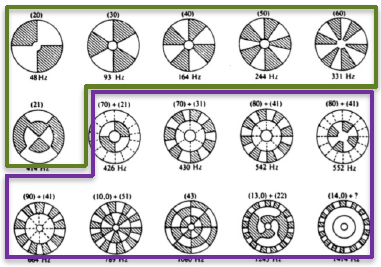
\includegraphics[height=0.2\textheight]{00_Images/08,09,10_chapter/08.png}} \hfill
    \subfloat[Measured mode shapes]{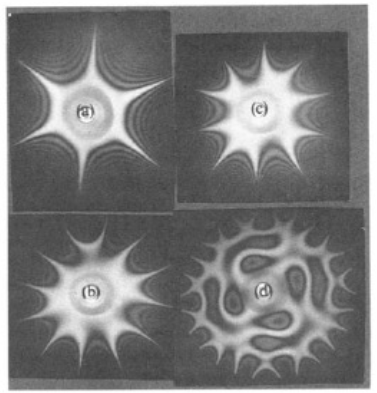
\includegraphics[height=0.2\textheight]{00_Images/08,09,10_chapter/09.png}}
    \caption{Comparison between theoretical and measured mode shapes}
    \label{fig:cymbalmode}
\end{figure}

\section{Cymbals Frequency Spectrum}

Modal frequencies are often approximated by a Chladni-like law in which the frequency depends on the nodal indices:
\[
f_{m,n} = c (m + 2n)^{p}
\]
Experiments indicate that a single slope does not fit the full modal set. Beyond a knee value \(m_c\), defined as a threshold in the number of nodal diameters, a different exponent and prefactor are required to follow the measured trend. This behavior is consistent with the fact that higher-order modes become more crowded and tend to exhibit stronger near-degeneracy and mixing, so the empirical scaling of \(f_{m,n}\) with \(m\) changes. A convenient representation is the piecewise model: 
\[
f_{m,n} =
\begin{cases}
c_1 (m + 2n)^{p_1}, & m \le m_c \\
c_2 (m + 2n)^{p_2}, & m > m_c
\end{cases}
\]

\section{Nonlinear and Transient Behavior}

\subsection{Spectral Evolution and Mode Coupling}

After a strike, cymbal sound evolves markedly over time. Nonlinear coupling among modes produces a large number of high-frequency partials, which are characteristic of cymbal timbre. Due to dispersion, high-frequency components can establish early, even before low-frequency standing-wave patterns become clearly recognizable. After an initial period that can be described as chaotic wave propagation, stable standing-wave patterns develop and correspond to the cymbal normal modes. Nonlinear phenomena may also favor the establishment of particular modal components, yielding an apparent pitch glide upward or downward, depending on the specific cymbal.

\subsection{Origin of the Nonlinearity}

A primary reason for strong nonlinear behavior is that the metal is thin, so tension and restoring forces are comparatively small. In this condition, the quadratic tension generated by modal displacements can have a large effect. Surface irregularities and hammering marks further facilitate coupling because abrupt spatial changes in displacement are known to ease energy exchange among modes.

\subsection{A Minimal Modal Picture}

A compact description treats each mode \(j\) as approximately sinusoidal with a slowly varying amplitude:
\[
y_j(t) = a_j(t) \sin(\omega_j t + \phi_j)
\]
For modes that are directly excited at the onset, a simple decay model is commonly assumed:
\[
a_i(t) = a_i \exp\left( - \frac{t}{\tau_i} \right)
\]
Upper modes may start with negligible energy and can grow through nonlinear coupling. In particular, energy transfer is emphasized when a near-integer relationship holds:
\[
\omega_j \approx n \omega_i
\]
In this picture, a coupled mode \(j\) may exhibit a delayed growth: its amplitude rises, reaches a maximum after a time \(t^\ast\), and then decays, consistent with the observed buildup and decay in different frequency bands:
\[
t^\ast = \frac{\tau_i \tau_j \ln\left( \tau_i / (n \tau_j) \right)}{\tau_i - n \tau_j}
\]
with the condition \( \tau_i > n \tau_j \). 

\section{Chaotic Vibration}

Cymbals behave as highly nonlinear systems: the fully developed sound after an arbitrary excitation depends strongly on chaotic behavior and cannot be easily described in detail. Even under sinusoidal excitation, a linear response is observed only for low amplitude forcing, whereas large amplitude forcing can suddenly establish additional frequencies associated with nonlinear interactions. Low-order modes can excite higher modes, which may combine and, in turn, drive further modes, yielding a cascade that sustains a chaotic regime before more stationary modal patterns become apparent.

\section{Tam-Tams}

Tam-tams can be regarded as oriental cymbals capable of producing very loud sounds. Their sound evolves strongly over time: it may begin with a very low-pitch impression and then nonlinearly build up higher and louder harmonics, raising the perceived pitch. Sustain can last for dozens of seconds. Higher harmonics vanish faster, and the late-time sound becomes dull again, similarly to the initial instants of vibration. A densely hammered surface enhances nonlinearities and contributes to this pronounced time evolution.

\section{Gongs}

Gongs share similarities with tam-tams but typically include a central dome. The dome strengthens tonal characteristics relative to tam-tams, and the first two axisymmetric modes often exhibit strong harmonic relationships. As for tam-tams, the spectrum becomes richer some time after the strike, consistent with the nonlinear buildup of additional components. The evolution can be described as a transition from a small number of prominent components at onset to a denser set of partials at intermediate times. 
